\documentclass[journal,12pt,twocolumn]{IEEEtran}

\usepackage{setspace}
\usepackage{gensymb}
\singlespacing
\usepackage[cmex10]{amsmath}

\usepackage{amsthm}

\usepackage{mathrsfs}
\usepackage{txfonts}
\usepackage{stfloats}
\usepackage{bm}
\usepackage{cite}
\usepackage{cases}
\usepackage{subfig}

\usepackage{longtable}
\usepackage{multirow}

\usepackage{float}

\usepackage{enumitem}
\usepackage{mathtools}
\usepackage{steinmetz}
\usepackage{tikz}
\usepackage{circuitikz}
\usepackage{verbatim}
\usepackage{tfrupee}
\usepackage[breaklinks=true]{hyperref}
\usepackage{graphicx}
\usepackage{tkz-euclide}
\usepackage[thinc]{esdiff}

\usetikzlibrary{calc,math}
\usepackage{listings}
    \usepackage{color}                                            %%
    \usepackage{array}                                            %%
    \usepackage{longtable}                                        %%
    \usepackage{calc}                                             %%
    \usepackage{multirow}                                         %%
    \usepackage{hhline}                                           %%
    \usepackage{ifthen}                                           %%
    \usepackage{lscape}     
\usepackage{multicol}
\usepackage{chngcntr}

\DeclareMathOperator*{\Res}{Res}

\renewcommand\thesection{\arabic{section}}
\renewcommand\thesubsection{\thesection.\arabic{subsection}}
\renewcommand\thesubsubsection{\thesubsection.\arabic{subsubsection}}

\renewcommand\thesectiondis{\arabic{section}}
\renewcommand\thesubsectiondis{\thesectiondis.\arabic{subsection}}
\renewcommand\thesubsubsectiondis{\thesubsectiondis.\arabic{subsubsection}}


\hyphenation{op-tical net-works semi-conduc-tor}
\def\inputGnumericTable{}                                 %%
\makeatletter
\setlength{\@fptop}{0pt}
\makeatother
\lstset{
%language=C,
frame=single, 
breaklines=true,
columns=fullflexible
}
\begin{document}

\newcommand{\BEQA}{\begin{eqnarray}}
\newcommand{\EEQA}{\end{eqnarray}}
\newcommand{\define}{\stackrel{\triangle}{=}}
\bibliographystyle{IEEEtran}
\raggedbottom
\setlength{\parindent}{0pt}
\providecommand{\mbf}{\mathbf}
\providecommand{\pr}[1]{\ensuremath{\Pr\left(#1\right)}}
\providecommand{\qfunc}[1]{\ensuremath{Q\left(#1\right)}}
\providecommand{\sbrak}[1]{\ensuremath{{}\left[#1\right]}}
\providecommand{\lsbrak}[1]{\ensuremath{{}\left[#1\right.}}
\providecommand{\rsbrak}[1]{\ensuremath{{}\left.#1\right]}}
\providecommand{\brak}[1]{\ensuremath{\left(#1\right)}}
\providecommand{\lbrak}[1]{\ensuremath{\left(#1\right.}}
\providecommand{\rbrak}[1]{\ensuremath{\left.#1\right)}}
\providecommand{\cbrak}[1]{\ensuremath{\left\{#1\right\}}}
\providecommand{\lcbrak}[1]{\ensuremath{\left\{#1\right.}}
\providecommand{\rcbrak}[1]{\ensuremath{\left.#1\right\}}}
\theoremstyle{remark}
\newtheorem{rem}{Remark}
\newcommand{\sgn}{\mathop{\mathrm{sgn}}}
\providecommand{\abs}[1]{\vert#1\vert}
\providecommand{\res}[1]{\Res\displaylimits_{#1}} 
\providecommand{\norm}[1]{\lVert#1\rVert}
%\providecommand{\norm}[1]{\lVert#1\rVert}
\providecommand{\mtx}[1]{\mathbf{#1}}
\providecommand{\mean}[1]{E[ #1 ]}
\providecommand{\fourier}{\overset{\mathcal{F}}{ \rightleftharpoons}}
%\providecommand{\hilbert}{\overset{\mathcal{H}}{ \rightleftharpoons}}
\providecommand{\system}{\overset{\mathcal{H}}{ \longleftrightarrow}}
	%\newcommand{\solution}[2]{\textbf{Solution:}{#1}}
\newcommand{\solution}{\noindent \textbf{Solution: }}
\newcommand{\cosec}{\,\text{cosec}\,}
\providecommand{\dec}[2]{\ensuremath{\overset{#1}{\underset{#2}{\gtrless}}}}
\newcommand{\myvec}[1]{\ensuremath{\begin{pmatrix}#1\end{pmatrix}}}
\newcommand{\mydet}[1]{\ensuremath{\begin{vmatrix}#1\end{vmatrix}}}
\numberwithin{equation}{subsection}
\makeatletter
\@addtoreset{figure}{problem}
\makeatother
\let\StandardTheFigure\thefigure
\let\vec\mathbf
\renewcommand{\thefigure}{\theproblem}
\def\putbox#1#2#3{\makebox[0in][l]{\makebox[#1][l]{}\raisebox{\baselineskip}[0in][0in]{\raisebox{#2}[0in][0in]{#3}}}}
     \def\rightbox#1{\makebox[0in][r]{#1}}
     \def\centbox#1{\makebox[0in]{#1}}
     \def\topbox#1{\raisebox{-\baselineskip}[0in][0in]{#1}}
     \def\midbox#1{\raisebox{-0.5\baselineskip}[0in][0in]{#1}}
\vspace{3cm}
\title{Assignment 7}
\author{Ananthoju Pranav Sai - AI20BTECH11004}
\maketitle
\newpage
\bigskip
\renewcommand{\thefigure}{\theenumi}
\renewcommand{\thetable}{\theenumi}
Download latex codes from 
%
Download all python codes from 
\begin{lstlisting}
https://github.com/Ananthoju-Pranav-Sai/AI1103/tree/main/Assignment_7_1/Codes
\end{lstlisting}
%
and latex codes from 
%
\begin{lstlisting}
https://github.com/Ananthoju-Pranav-Sai/AI1103/blob/main/Assignment_7_1/main.tex
\end{lstlisting}
\section*{STATS P1 IESISS19 Q 31}
Let X be a random variable with p.d.f
\begin{align}
    f_{X}(x)=\begin{cases} 
            \frac{2x}{\pi^2}  &  0<x<\pi\\
            0 & \text{otherwise}
            \end{cases} 
\end{align}
Let Y = $\sin{X}$, then for $0<y<1$, the p.d.f of Y is given by,\\
\begin{enumerate}[label = (\Alph*)]
    \item  $\frac{2\pi}{\sqrt{1-y^2}}$\\
    \item  $\frac{\pi}{2}\sqrt{1-y^2}$\\
    \item  $\frac{2}{\pi}\sqrt{1-y^2}$\\
    \item  $\frac{2}{\pi\sqrt{1-y^2}}$
\end{enumerate}
\section*{Solution}
Given p.d.f of X as
\begin{align}
    f_{X}(x)=\begin{cases} 
            \frac{2x}{\pi^2}  &  0<x<\pi\\
            0 & \text{otherwise}
            \end{cases} 
\end{align}
\begin{align}
    F_X(x) &= \pr{X\leq x}\\
    \implies F_X(x) &= \int_{-\infty}^{x}f_X(t)\,dt
\end{align}
which can be written as
\begin{align}
    F_{X}(x)=\begin{cases} 
            0 & x\le 0\\
            \frac{x^2}{\pi^2}  &  0<x<\pi\\
            1 & x\ge \pi
            \end{cases}
            \label{a}
\end{align}
Now c.d.f of $Y$ can be written as 
\begin{align}
    F_Y(y) &= \pr{Y\leq y}\\
    \implies F_Y(y) &= \pr{\sin{X}\leq y}
\end{align}
As $X\in(0,\pi)$, $\sin{X}\leq y$ has two solutions i.e., either
 $X\leq \sin^{-1}{y}$ or $X\geq \pi-\sin^{-1}{y}$ as shown in \ref{plot}
 \begin{figure}[H]
     \centering
     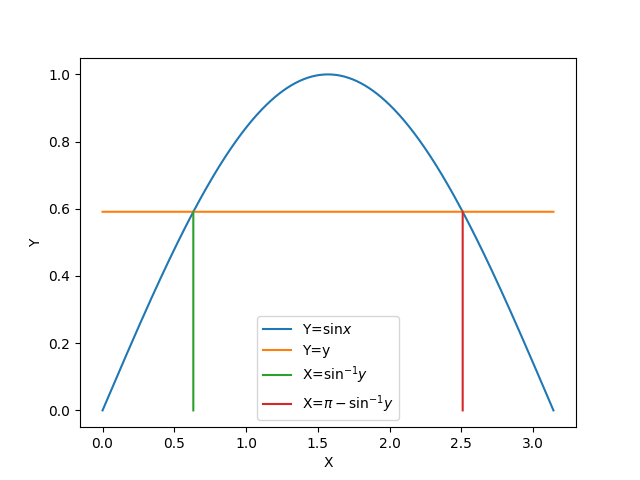
\includegraphics[width=\linewidth]{plot.png}
     \caption{$Y=\sin X$ plot}
     \label{plot}
 \end{figure}
\begin{align}
    \implies F_Y(y) &= \pr{X\leq \sin^{-1}{y}}+\pr{X\geq \pi-\sin^{-1}{y}}\\
    \implies F_Y(y) &= F_X(\sin^{-1}{y})+1-\pr{X\leq \pi-\sin^{-1}{y}}\\
    \implies F_Y(y) &= F_X(\sin^{-1}{y})+1-F_X(\pi-\sin^{-1}{y})
    \label{b}
\end{align}
using \eqref{a} in \eqref{b}
\begin{align}
    \implies F_Y(y) &= \frac{\brak{\sin^{-1}{y}}^2}{\pi^2}+1-\frac{\brak{\pi-\sin^{-1}{y}}^2}{\pi^2}\\
    \implies F_Y(y) &= \frac{2\sin^{-1}{y}}{\pi}
\end{align}
Now pdf of Y can be written as
\begin{align}
     f_Y(y) &= \diff{F_Y(y)}{y}\\
    \implies f_Y(y) &= \frac{2}{\pi}\diff{\brak{\sin^{-1}{y}}}{y}\\
    \implies f_Y(y) &= \frac{2}{\pi\sqrt{1-y^2}}
\end{align}
Hence, option(D) is correct.
\end{document}